% Overview slides for the Iliad Intensive worksheets:
%   - Solomonoff Induction  (solomonoff-all.tex, Leon Lang)
%   - AIXI                  (aixi-worksheet.tex, David Quarel)
% Template cribbed from ../arena-intro-rl-slides/main.tex
%
% Build: pdflatex -interaction=nonstopmode -halt-on-error iliad-david1-slides.tex  (twice)

\documentclass[10pt,aspectratio=169,handout]{beamer}
\usepackage[utf8]{inputenc}
\usepackage{amsmath}
\usepackage{amsfonts}
\usepackage{amssymb}
\usepackage{graphicx}
\usetheme{Madrid}
\usepackage{stmaryrd}
\usepackage{xcolor}
\usepackage{tikz}
\usetikzlibrary{calc, positioning, arrows.meta, shapes.geometric}

\hypersetup{
    colorlinks=true,
    linkcolor=white,
    urlcolor=cyan,
}
\urlstyle{same}

%====================== macros shared with the worksheets ======================
\newcommand{\cA}{\mathcal{A}}
\newcommand{\cO}{\mathcal{O}}
\newcommand{\cR}{\mathcal{R}}
\newcommand{\cE}{\mathcal{E}}
\newcommand{\cH}{\mathcal{H}}
\newcommand{\cM}{\mathcal{M}}
\newcommand{\Mc}{\mathcal{M}}
\newcommand{\Ex}{\mathbb{E}}
\newcommand{\Prob}{\mathbb{P}}
\newcommand{\B}{\mathbb{B}}
\DeclareMathOperator*{\argmax}{arg\,max}
\newcommand{\TV}{\mathrm{TV}}
\newcommand{\KL}{\mathrm{KL}}
\newcommand{\aes}{{\text{\ae}}}            % action--percept history symbol
\newcommand{\red}[1]{\textcolor{red}{#1}}
\newcommand{\blue}[1]{\textcolor{blue}{#1}}
\newcommand{\iver}[1]{\llbracket #1 \rrbracket}

%===============================================================================
\begin{document}

\title[Solomonoff \& AIXI: a speedrun]{Universal AI: Solomonoff Induction \& AIXI \\ \small A whirlwind overview of the two worksheets}
\author[Lang \& Quarel]{Leon Lang \quad David Quarel}
\institute[Iliad / LISA]{Iliad Intensive \,---\, London Initiative for Safe AI}
\date{April 2026}

\frame{\titlepage}

%===============================================================================
\begin{frame}{The big picture: one agent, two halves}
\begin{itemize}
    \item \textbf{Universal AI} asks: what would an \emph{optimally intelligent} agent look like, given unlimited compute and the weakest possible assumptions?
    \pause
    \item It splits into two problems:
    \begin{enumerate}
        \item \textbf{Prediction (Solomonoff):} passively observe a sequence $x_1, x_2, \ldots$ and predict the next symbol. \emph{How should you learn?}
        \pause
        \item \textbf{Action (AIXI):} interact with an unknown environment, take actions, collect reward. \emph{How should you act?}
    \end{enumerate}
    \pause
    \item \textbf{The common engine:} a single \textbf{Bayesian mixture} $\xi$ over a class $\cM$ of candidate environments, weighted by a prior $w_\nu$.
    \begin{itemize}
        \item Solomonoff: $\xi$ \emph{predicts} as well as the truth $\mu$.
        \item AIXI: the Bayes-optimal policy $\pi_\xi^*$ \emph{acts} as well as if it knew $\mu$.
    \end{itemize}
    \pause
    \item \textbf{Universal} choice: $\cM=$ all computable environments, prior $w_\nu = 2^{-K(\nu)}$ (shorter programs preferred). Assumption ``$\mu\in\cM$'' becomes ``\emph{the universe is computable}''.
\end{itemize}
\end{frame}

%========================= PART 1: SOLOMONOFF ==================================
\begin{frame}
\begin{center}
{\Huge \textbf{Part I: Solomonoff Induction}}\\[1em]
{\large \emph{Learning to predict}}\\[2em]
\end{center}
\centering\small (worksheet by Leon Lang)
\end{frame}

\begin{frame}{The problem of induction, formalized}
\begin{itemize}
    \item A true (unknown) environment $\mu$ generates a binary sequence; each bit
    $x_t \sim \mu(\cdot \mid x_{<t})$.
    \pause
    \item A \textbf{predictor} $P$ sees the past $x_{<t}$ and outputs a distribution
    $P(\cdot \mid x_{<t})$ over the next bit.
    \pause
    \item \textbf{Quality measure:} total $\mu$-expected squared prediction error
    \[
    S_\infty^\mu := \sum_{t=1}^{\infty} \sum_{x_{<t}} \mu(x_{<t})
        \sum_{x_t \in \B} \big( P(x_t \mid x_{<t}) - \mu(x_t \mid x_{<t}) \big)^2.
    \]
    \pause
    \item \textbf{Goal:} build a $P$ making $S_\infty^\mu$ \emph{small} --- even though $\mu$ is unknown!
    \pause
    \item \textbf{Idea:} don't bet on one model. Mix over a whole class $\cM=\{\nu_1,\nu_2,\dots\}$.
\end{itemize}
\end{frame}

\begin{frame}{The Bayesian mixture $\xi$}
\begin{block}{Definition}
Class $\cM=\{\nu_1,\nu_2,\dots\}$ with prior weights $w_\nu>0$, $\sum_\nu w_\nu = 1$.
\[
\xi(x_{1:t}) := \sum_{\nu \in \cM} w_\nu\, \nu(x_{1:t}).
\]
\end{block}
\pause
\begin{itemize}
    \item \textbf{Key fact (mixture is a predictor):} its one-step prediction is a
    \emph{posterior-weighted} average of the members' predictions,
    \[
    \xi(x_t \mid x_{<t}) = \sum_{\nu \in \cM} w(\nu \mid x_{<t})\, \nu(x_t \mid x_{<t}),
    \qquad
    w(\nu \mid x_{<t}) = w_\nu\,\frac{\nu(x_{<t})}{\xi(x_{<t})}.
    \]
    \pause
    \item Posterior weights sum to $1$ $\Rightarrow$ $\xi(\cdot\mid x_{<t})$ is a genuine distribution.
    \pause
    \item \textbf{Posterior update is multiplicative:}
    $w(\nu \mid x_{1:t}) = w(\nu\mid x_{<t})\cdot \dfrac{\nu(x_t\mid x_{<t})}{\xi(x_t\mid x_{<t})}$
    --- reweight by how well $\nu$ just predicted. (Bayes' rule!)
\end{itemize}
\end{frame}

\begin{frame}{Two more ingredients}
\begin{block}{Dominance}
Dropping all but one term, $\;\xi(x_{1:t}) \geq w_\nu\, \nu(x_{1:t})\;$ for every $\nu \in \cM$.\\
So $\mu(x_{1:t})/\xi(x_{1:t}) \leq 1/w_\mu$: \emph{the mixture never assigns much less mass than the truth.}
\end{block}
\pause
\begin{block}{KL divergence telescopes}
Cumulative KL over a history splits into a sum of per-step KLs:
\[
D_n(\nu \parallel \rho) = \sum_{t=1}^n d_t(\nu \parallel \rho).
\]
\end{block}
\pause
\begin{block}{Pinsker's inequality (binary)}
Squared error is controlled by KL:
$\displaystyle \sum_{x}(q_x - p_x)^2 \leq \sum_x p_x \ln \tfrac{p_x}{q_x}.$
\end{block}
\end{frame}

\begin{frame}{Main result: the cumulative prediction bound}
Chain the three ingredients together:
\[
S^\mu_\infty
\;\overset{\text{Pinsker}}{\leq}\;
D^\mu_\infty
\;\overset{\text{dominance}}{\leq}\;
\lim_{n\to\infty}\sum_{x_{1:n}}\mu(x_{1:n})\ln\tfrac{1}{w_\mu}
\;=\;
-\ln w_\mu .
\]
\pause
\begin{block}{Cumulative bound}
\[
\boxed{\;S^\mu_\infty \;\leq\; -\ln w_\mu\;}
\]
\end{block}
\begin{itemize}
    \item Total squared error over \emph{all time} is finite, bounded by the prior penalty on $\mu$.
    \item Higher prior on the truth $\Rightarrow$ smaller total error. \emph{Errors are summable} --- so per-step error $\to 0$.
\end{itemize}
\end{frame}

\begin{frame}{Specializing to the Solomonoff prior}
\begin{itemize}
    \item Take the \textbf{Solomonoff prior} $w_\nu = 2^{-K(\nu)}$, where $K(\nu)$ is the
    \emph{Kolmogorov complexity} --- length of the shortest program computing $\nu$.
    \pause
    \item Substitute $w_\mu = 2^{-K(\mu)}$ into the cumulative bound:
\end{itemize}
\begin{block}{Explicit complexity bound}
\[
\boxed{\; S^\mu_\infty \;\leq\; K(\mu)\,\ln 2 \;}
\]
\end{block}
\pause
\begin{itemize}
    \item \textbf{Interpretation:} the total prediction error is bounded by the
    \emph{description length} of the true environment. Simpler worlds are learned faster.
    \item This is the formal version of \textbf{Occam's razor}.
\end{itemize}
\end{frame}

\begin{frame}{What else the worksheet proves}
\begin{itemize}
    \item \textbf{Bounded mistakes:} on a deterministic sequence, the ``predict-the-likelier-bit''
    rule makes at most $-2\ln w_\mu$ wrong guesses --- \emph{ever}.
    \pause
    \item \textbf{Pareto optimality:} no other predictor beats $\xi$ on \emph{every} $\nu\in\cM$
    simultaneously (for KL loss \emph{and} squared loss). Via a Pythagorean / Bregman identity.
    \pause
    \item \textbf{Misspecification ($\mu \notin \cM$):} the bound degrades gracefully,
    \[
    S^\mu_\infty \lesssim -\ln w_{\hat\mu} + D_n(\mu \parallel \hat\mu),
    \]
    where $\hat\mu$ is the closest model in $\cM$ to $\mu$. A constant term $+$ an approximation term.
\end{itemize}
\end{frame}

%========================= PART 2: AIXI ========================================
\begin{frame}
\begin{center}
{\Huge \textbf{Part II: AIXI}}\\[1em]
{\large \emph{Learning to act}}\\[2em]
\end{center}
\centering\small (worksheet by David Quarel)
\end{frame}

\begin{frame}{From prediction to action}
\begin{itemize}
    \item Now the agent doesn't just watch --- it \textbf{acts}, and its actions shape what it sees.
    \pause
    \item At each step $t$: the agent picks action $a_t$, the environment returns a
    \textbf{percept} $e_t=(o_t,r_t)$ = observation $+$ reward.
    \[
    \underbrace{a_1\, e_1}_{\text{step }1}\; a_2\, e_2 \; a_3\, e_3 \;\cdots \qquad
    (\text{history } \aes_{<t})
    \]
    \pause
    \item Spaces: actions $\cA$, observations $\cO$, rewards $\cR \subset [0,1]$, percepts $\cE=\cO\times\cR$.
    \pause
    \item \textbf{No Markov / MDP assumption!} The environment may depend on the \emph{entire history}
    --- this is much more general than the RL setting (states, $T$, $R$).
\end{itemize}
\end{frame}

\begin{frame}{The three players}
\begin{block}{Policy $\pi$}
$\pi(a_t \mid \aes_{<t})$ --- agent's distribution over the next action given history.
\end{block}
\pause
\begin{block}{Environment $\nu$}
$\nu(e_t \mid \aes_{<t}\, a_t)$ --- distribution over the next percept. True one is $\mu$.
\end{block}
\pause
\begin{block}{Interaction measure $\nu^\pi$}
Run $\pi$ inside $\nu$ and multiply along the history:
\[
\nu^\pi(\aes_{t:m} \mid \aes_{<t}) := \prod_{k=t}^m \pi(a_k\mid \aes_{<k})\,\nu(e_k\mid \aes_{<k}a_k).
\]
\end{block}
\pause
\textbf{Factorization:} $\nu^\pi = \pi \cdot \nu$ --- the policy factor is the same for every $\nu$, so it \emph{cancels} when comparing environments. This is what makes everything reduce to the prediction problem.
\end{frame}

\begin{frame}{Value, optimality, and AIXI}
\begin{block}{Value function (geometric discount $\gamma$)}
\[
V_\nu^{\pi}(\aes_{<t}) := (1-\gamma)\,\Ex_\nu^\pi\!\Big[\textstyle\sum_{k\geq t} \gamma^{k-t} r_k \;\Big|\; \aes_{<t}\Big] \in [0,1].
\]
\end{block}
\pause
\begin{itemize}
    \item \textbf{Optimal value} $V_\nu^* := \sup_\pi V_\nu^\pi$; an optimal policy $\pi_\nu^*$ attains it
    (exists, via Bellman + backward induction).
    \item \textbf{Bayes-optimal policy} $\pi_\xi^* \in \argmax_\pi V_\xi^\pi$ --- acts optimally w.r.t.\ the \emph{mixture}.
\end{itemize}
\pause
\begin{block}{AIXI}
$\pi_\xi^*$ with $\cM=$ all lower-semicomputable environments and prior $w_\nu = 2^{-K(\nu)}$.
\emph{The Bayes-optimal agent under Occam's razor.}
\end{block}
\end{frame}

\begin{frame}{Key structural properties of $V$}
\begin{block}{Linearity of $V^\pi$ in the environment}
\[
V_\xi^\pi(\aes_{<t}) = \sum_{\nu\in\cM} w(\nu\mid \aes_{<t})\, V_\nu^\pi(\aes_{<t}).
\]
The mixture's value is the posterior average of the members' values.
\end{block}
\pause
\begin{block}{Dominance of value}
$\xi^\pi(\aes_{1:m}) \geq w_\nu\, \nu^\pi(\aes_{1:m})$ --- the mixture covers every environment.
\end{block}
\pause
\textbf{Caveat:} $V_\xi^*$ (optimal value) is only \emph{convex}, not linear --- one policy must do well across all $\nu$ at once. (E.g.\ predicting a two-headed vs.\ two-tailed coin: each is trivial alone, the mixture is a fair coin.)
\end{frame}

\begin{frame}{The three main AIXI results}
\begin{center}
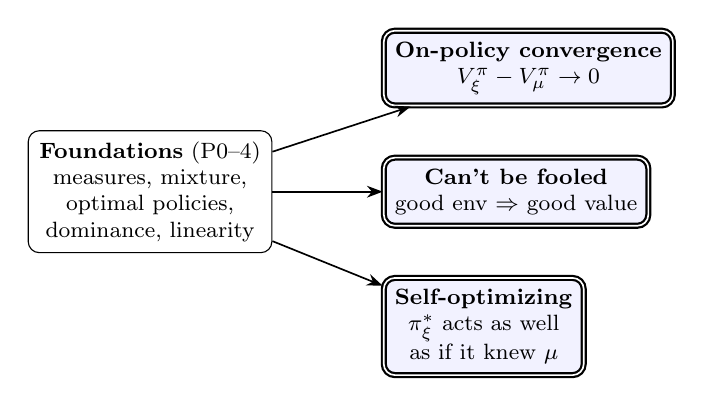
\begin{tikzpicture}[
    node distance=6mm and 10mm,
    box/.style={draw, rounded corners, align=center, font=\footnotesize, inner sep=4pt, minimum height=8mm},
    main/.style={box, thick, double, fill=blue!5},
    arr/.style={-{Stealth}, semithick}
]
\node[box] (f) {\textbf{Foundations} (P0--4)\\ measures, mixture,\\ optimal policies,\\ dominance, linearity};
\node[main, above right=3mm and 14mm of f] (r1) {\textbf{On-policy convergence}\\ $V_\xi^\pi - V_\mu^\pi \to 0$};
\node[main, right=14mm of f] (r2) {\textbf{Can't be fooled}\\ good env $\Rightarrow$ good value};
\node[main, below right=3mm and 14mm of f] (r3) {\textbf{Self-optimizing}\\ $\pi_\xi^*$ acts as well\\ as if it knew $\mu$};
\draw[arr] (f) -- (r1);
\draw[arr] (f) -- (r2);
\draw[arr] (f) -- (r3);
\end{tikzpicture}
\end{center}
\begin{itemize}\footnotesize
    \item All three: the Bayesian agent inherits the guarantees it would have if it knew the truth.
    \item Result~3 needs heavier machinery (martingales, change of measure) --- a stretch goal.
\end{itemize}
\end{frame}

\begin{frame}{Result 1: On-policy value convergence}
\begin{block}{Theorem}
For any $\mu\in\cM$ and any policy $\pi$,
\[
V_\xi^\pi(\aes_{<t}) - V_\mu^\pi(\aes_{<t}) \;\to\; 0 \qquad \mu^\pi\text{-almost surely}.
\]
\end{block}
\pause
\textbf{Proof skeleton:}
\begin{enumerate}
    \item Value differences are bounded by \textbf{total variation}: $|V_\xi^{\pi,m}-V_\mu^{\pi,m}| \leq \TV(\xi^\pi,\mu^\pi)$.
    \pause
    \item Dominance $\Rightarrow$ $\xi^\pi$ \emph{covers} $\mu^\pi$.
    \pause
    \item \textbf{Blackwell--Dubins} (merging of opinions): if $Q$ covers $P$, their TV distance $\to 0$, $P$-a.s.
\end{enumerate}
\pause
\emph{The mixture learns to evaluate any fixed policy exactly as the true environment would.}
\end{frame}

\begin{frame}{Result 2: AIXI can't be fooled}
\begin{block}{Theorem (deterministic $\mu$)}
If the truth is reachable-good, $V_\mu^*(\aes_{<t}) > \varepsilon$ along the played history, then
\[
V_\xi^*(\aes_{<t}) \;\geq\; w_\mu\,\varepsilon \;>\; 0 .
\]
\end{block}
\pause
\textbf{Two short steps:}
\begin{itemize}
    \item By linearity, plugging in $\pi_\mu^*$ and dropping all but the $\mu$ term:
    $V_\xi^*(\aes_{<t}) \geq w(\mu\mid \aes_{<t})\, V_\mu^*(\aes_{<t})$.
    \pause
    \item For deterministic $\mu$, the posterior never shrinks: $w(\mu\mid \aes_{<t}) \geq w_\mu$.
\end{itemize}
\pause
\emph{Whenever good behaviour is achievable, the Bayes-optimal agent secures non-trivial value --- it cannot be tricked into giving up.}
\end{frame}

\begin{frame}{Result 3: Self-optimizing property (stretch goal)}
\begin{block}{Theorem (finite $\cM$)}
If \emph{some} policy can learn to act optimally in every $\nu\in\cM$, then $\pi_\xi^*$ does too:
\[
V_\mu^*(\aes_{<t}) - V_\mu^{\pi_\xi^*}(\aes_{<t}) \to 0 \quad \mu^\pi\text{-a.s.}
\]
\end{block}
\pause
\textbf{Engine: likelihood ratios are martingales.}
\begin{itemize}
    \item $X_{\nu,t} := \nu(\aes_{1:t})/\mu(\aes_{1:t})$ is a non-negative $\mu^\pi$-martingale.
    \pause
    \item \textbf{Doob} $\Rightarrow$ it converges. Split environments into:
    \emph{ruled out} ($X_{\nu,\infty}=0$, posterior vanishes) vs.\ \emph{still plausible} ($X_{\nu,\infty}>0$).
    \pause
    \item \textbf{Change of measure} (Markov inequality) transfers convergence between $\nu$ and $\mu$.
\end{itemize}
\pause
\emph{This is the central justification for AIXI: learning to predict $\Rightarrow$ learning to act.}
\end{frame}

%========================= WRAP-UP ============================================
\begin{frame}{The two sheets, side by side}
\small
\begin{center}
\renewcommand{\arraystretch}{1.4}
\begin{tabular}{l|l|l}
 & \textbf{Solomonoff} & \textbf{AIXI} \\\hline
Setting & passive prediction & active interaction \\
Data & sequence $x_{1:t}$ & history $\aes_{<t}$ (actions + percepts) \\
Engine & mixture $\xi(x_{1:t})=\sum_\nu w_\nu \nu$ & same, with policies: $\xi^\pi = \pi\cdot\xi$ \\
Tool & dominance, KL, Pinsker & dominance, linearity, TV, martingales \\
Guarantee & $S^\mu_\infty \leq -\ln w_\mu$ & $V_\xi^\pi \to V_\mu^\pi$; self-optimizing \\
Universal & $w_\nu = 2^{-K(\nu)} \Rightarrow K(\mu)\ln 2$ & $\cM=$ all comp.\ env., $w_\nu=2^{-K(\nu)}$ \\
\end{tabular}
\end{center}
\pause
\begin{itemize}
    \item \textbf{One idea throughout:} a dominant Bayesian mixture inherits the truth's guarantees, up to a prior penalty $-\ln w_\mu$.
    \item \textbf{Universality:} pick the prior $2^{-K(\nu)}$ and the penalty becomes the truth's description length.
\end{itemize}
\end{frame}

\begin{frame}{Takeaways}
\begin{itemize}
    \item \textbf{Solomonoff} solves induction: mix over all computable hypotheses, weighted by simplicity.
    Total prediction error $\leq K(\mu)\ln 2$.
    \pause
    \item \textbf{AIXI} lifts this to action: the Bayes-optimal policy over the same universal mixture.
    It learns to predict \emph{and} to act as well as if it knew the world.
    \pause
    \item \textbf{The catch:} both are \emph{incomputable} ($K$ is uncomputable; $\cM$ is uncountable to search).
    They are gold standards, not algorithms --- and the prior's universal-Turing-machine dependence
    can be adversarially abused.
    \pause
    \item \textbf{Why care for safety:} a precise, assumption-light model of idealized intelligence ---
    a target to approximate, and a lens on what optimal agents do.
\end{itemize}
\vspace{1em}
\begin{center}
\large Questions? \quad $\longrightarrow$ \quad open the worksheets.
\end{center}
\end{frame}

\end{document}
